\documentclass[8pt,aspectratio=169]{beamer}
\usepackage[utf8]{inputenc}
\usepackage{graphicx}
\usepackage{amsmath,amssymb}
\usepackage{algorithm2e}
\usepackage{listings}
\usepackage{xcolor}
\usepackage{tikz}
\usepackage{pgfplots}
\pgfplotsset{compat=1.17}
\usepackage{subfigure}
\usepackage{hyperref}
\usepackage{tcolorbox}

% Theme settings
\usetheme{Frankfurt}
\usecolortheme{seahorse}
\setbeamertemplate{navigation symbols}{}
\setbeamertemplate{footline}[frame number]

% Custom colors
\definecolor{darkblue}{RGB}{0,51,102}
\definecolor{lightblue}{RGB}{173,216,230}
\definecolor{codegreen}{RGB}{0,128,0}
\definecolor{codegray}{RGB}{150,150,150}
\definecolor{codepurple}{RGB}{128,0,128}
\definecolor{backcolor}{RGB}{245,245,245}

% Pedagogical boxes
\newtcolorbox{checkpoint}{
    colback=yellow!10,
    colframe=yellow!50!black,
    title={\textbf{Checkpoint}},
    fonttitle=\bfseries
}

\newtcolorbox{intuition}{
    colback=purple!10,
    colframe=purple!50!black,
    title={\textbf{Intuition}},
    fonttitle=\bfseries
}

\newtcolorbox{realworld}{
    colback=orange!10,
    colframe=orange!50!black,
    title={\textbf{Real World}},
    fonttitle=\bfseries
}

\newtcolorbox{misconception}{
    colback=red!10,
    colframe=red!50!black,
    title={\textbf{Common Misconception}},
    fonttitle=\bfseries
}

% Code listing settings
\lstset{
    backgroundcolor=\color{backcolor},
    basicstyle=\ttfamily\footnotesize,
    breakatwhitespace=false,
    breaklines=true,
    captionpos=b,
    commentstyle=\color{codegreen},
    keywordstyle=\color{blue},
    numberstyle=\tiny\color{codegray},
    stringstyle=\color{codepurple},
    showstringspaces=false,
    frame=single,
    numbers=left,
    language=Python
}

% Include slide layouts
% SLIDE LAYOUT TEMPLATES FOR NLP COURSE
% Three consistent layouts used throughout the course

% ==============================================================
% LAYOUT 1: CONCEPT SLIDE
% Used for: Theory, definitions, mathematical concepts
% Features: Title, main content area with bullets/equations, optional figure
% ==============================================================

\newcommand{\conceptslide}[3]{ % #1: title, #2: content, #3: optional figure
\begin{frame}[t]{#1}
    \begin{columns}[T]
        \begin{column}{0.6\textwidth}
            #2
        \end{column}
        \begin{column}{0.35\textwidth}
            \centering
            #3
        \end{column}
    \end{columns}
\end{frame}
}

% ==============================================================
% LAYOUT 2: CODE & IMPLEMENTATION SLIDE
% Used for: Code examples, algorithms, implementation details
% Features: Title, code block, explanation text
% ==============================================================

% Note: For code slides, use \begin{frame}[fragile] manually

\newcommand{\codeexplanation}[1]{%
    \vspace{0.5em}
    \small
    #1
}

\newcommand{\codeblock}[2][Python]{%
    \begin{lstlisting}[language=#1, basicstyle=\ttfamily\tiny]
#2
    \end{lstlisting}
}

\newcommand{\codeslide}[3]{%
    \begin{frame}[fragile]{#1}
    \begin{columns}[T]
        \column{0.55\textwidth}
        \codeblock{#2}
        \column{0.43\textwidth}
        \codeexplanation{#3}
    \end{columns}
    \end{frame}
}

% ==============================================================
% LAYOUT 3: RESULTS & VISUALIZATION SLIDE
% Used for: Experimental results, charts, comparisons
% Features: Title, large visualization area, key insights
% ==============================================================

\newcommand{\resultslide}[3]{ % #1: title, #2: visualization, #3: insights
\begin{frame}[t]{#1}
    \centering
    \vspace{-0.5em}
    #2
    \vspace{0.5em}
    
    \begin{block}{Key Insights}
        #3
    \end{block}
\end{frame}
}

% Additional utility commands for consistency

% Highlighted text
\newcommand{\highlight}[1]{\textcolor{blue}{\textbf{#1}}}

% Math notation shortcuts
\newcommand{\prob}[1]{P(#1)}
\newcommand{\given}{\mid}
\newcommand{\argmax}{\operatorname{argmax}}
\newcommand{\softmax}{\operatorname{softmax}}

% Standard figure size
\newcommand{\stdfigsizeinchins}{0.4\textwidth}

% For code blocks, use lstlisting directly:
% \begin{lstlisting}[language=Python]
% ... code ...
% \end{lstlisting}

% Equation highlight box
\newcommand{\eqbox}[1]{
    \begin{center}
    \colorbox{lightblue!20}{
        \parbox{0.8\textwidth}{
            \vspace{0.3em}
            \centering
            #1
            \vspace{0.3em}
        }
    }
    \end{center}
}

\title[Week 6: Pre-trained Models]{Natural Language Processing}
\subtitle{Week 6: Pre-trained Language Models - Simplified Edition}
\author{Joerg R. Osterrieder}
\date{}

\begin{document}

% Title page
\begin{frame}
    \titlepage
\end{frame}

\section{Week 6: Pre-trained Language Models}

% Opening hook with analogy
\begin{frame}[t]{The Reading Revolution: A Story}
    \begin{columns}
    \column{0.5\textwidth}
    \textbf{Imagine two students:}
    
    \vspace{0.5em}
    \textbf{Student A:} Never learned to read
    \begin{itemize}
        \item Starts medical school
        \item Must learn alphabet first
        \item Then words, grammar, sentences
        \item Finally can read medical texts
        \item Takes 10 years to become doctor
    \end{itemize}
    
    \vspace{0.5em}
    \textbf{Student B:} Already knows how to read
    \begin{itemize}
        \item Starts medical school
        \item Focuses only on medical knowledge
        \item Becomes doctor in 4 years
    \end{itemize}
    
    \column{0.5\textwidth}
    \begin{center}
    \includegraphics[width=\textwidth]{../figures/transfer_learning_landscape.pdf}
    \end{center}
    
    \begin{intuition}
    Pre-training is like teaching AI to read before teaching it specific tasks!
    \end{intuition}
    \end{columns}
\end{frame}

% Learning objectives with icons
\begin{frame}[t]{Your Learning Journey Today}
    \begin{columns}
    \column{0.6\textwidth}
    \textbf{By the end of this session, you will:}
    
    \vspace{0.5em}
    \begin{enumerate}
        \item \textbf{Understand} why we pre-train models
        \begin{itemize}
            \item The waste problem
            \item Transfer learning magic
        \end{itemize}
        
        \item \textbf{Master} two approaches
        \begin{itemize}
            \item BERT: Fill in the blanks
            \item GPT: Predict what's next
        \end{itemize}
        
        \item \textbf{Apply} fine-tuning
        \begin{itemize}
            \item Adapt to your task
            \item 10x faster than training from scratch
        \end{itemize}
        
        \item \textbf{Choose} the right model
        \begin{itemize}
            \item Decision tree for model selection
            \item Trade-offs and considerations
        \end{itemize}
    \end{enumerate}
    
    \column{0.4\textwidth}
    \begin{checkpoint}
    Think of pre-training like learning to drive: Once you know how, you can drive any car, not just the one you learned in!
    \end{checkpoint}
    
    \vspace{1em}
    \begin{realworld}
    Every time you use autocomplete on your phone, you're using a pre-trained model!
    \end{realworld}
    \end{columns}
\end{frame}

% The problem visualization
\begin{frame}[t]{The Million Dollar Waste}
    \begin{columns}
    \column{0.5\textwidth}
    \textbf{The Old Way (2017):}
    
    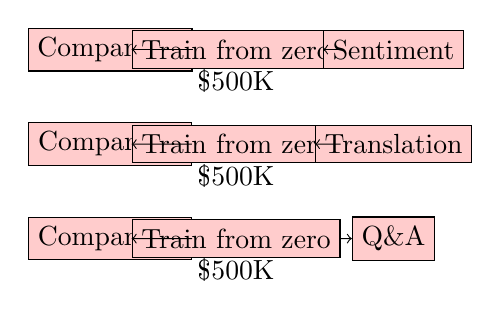
\begin{tikzpicture}[scale=0.8]
        % Company A
        \node[draw, rectangle, fill=red!20] (a1) at (0,0) {Company A};
        \node[draw, rectangle, fill=red!20] (a2) at (2,0) {Train from zero};
        \node[draw, rectangle, fill=red!20] (a3) at (4.5,0) {Sentiment};
        \draw[->] (a1) -- (a2);
        \draw[->] (a2) -- (a3);
        \node at (2,-0.5) {\$500K};
        
        % Company B
        \node[draw, rectangle, fill=red!20] (b1) at (0,-1.5) {Company B};
        \node[draw, rectangle, fill=red!20] (b2) at (2,-1.5) {Train from zero};
        \node[draw, rectangle, fill=red!20] (b3) at (4.5,-1.5) {Translation};
        \draw[->] (b1) -- (b2);
        \draw[->] (b2) -- (b3);
        \node at (2,-2) {\$500K};
        
        % Company C
        \node[draw, rectangle, fill=red!20] (c1) at (0,-3) {Company C};
        \node[draw, rectangle, fill=red!20] (c2) at (2,-3) {Train from zero};
        \node[draw, rectangle, fill=red!20] (c3) at (4.5,-3) {Q\&A};
        \draw[->] (c1) -- (c2);
        \draw[->] (c2) -- (c3);
        \node at (2,-3.5) {\$500K};
    \end{tikzpicture}
    
    \textbf{Total waste: \$1.5 million!}
    
    \column{0.5\textwidth}
    \textbf{The Smart Way (Today):}
    
    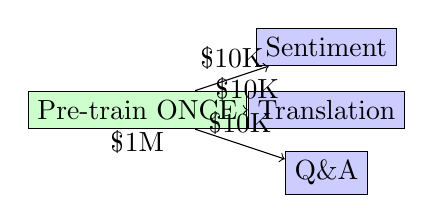
\begin{tikzpicture}[scale=0.8]
        % Pre-training
        \node[draw, rectangle, fill=green!20] (pre) at (1,0) {Pre-train ONCE};
        \node at (1,-0.5) {\$1M};
        
        % Companies
        \node[draw, rectangle, fill=blue!20] (a) at (4,1) {Sentiment};
        \node[draw, rectangle, fill=blue!20] (b) at (4,0) {Translation};
        \node[draw, rectangle, fill=blue!20] (c) at (4,-1) {Q\&A};
        
        \draw[->] (pre) -- (a) node[midway,above] {\$10K};
        \draw[->] (pre) -- (b) node[midway,above] {\$10K};
        \draw[->] (pre) -- (c) node[midway,above] {\$10K};
    \end{tikzpicture}
    
    \textbf{Total cost: \$1.03 million}
    \textbf{Savings: \$470,000!}
    
    \begin{misconception}
    ``Pre-training is just memorizing text'' - No! It's learning language patterns, grammar, and world knowledge that transfers to any task.
    \end{misconception}
    \end{columns}
\end{frame}

% BERT explained simply
\begin{frame}[t]{BERT: The Fill-in-the-Blank Master}
    \begin{columns}
    \column{0.5\textwidth}
    \textbf{How BERT Learns:}
    
    \begin{center}
    \includegraphics[width=\textwidth]{../figures/bert_masking_visualization.pdf}
    \end{center}
    
    \textbf{Like a comprehension test:}
    \begin{enumerate}
        \item Take a sentence
        \item Hide some words (15\%)
        \item Guess the hidden words
        \item Use ALL surrounding context
    \end{enumerate}
    
    \column{0.5\textwidth}
    \textbf{Try it yourself:}
    
    ``The [MASK] sat on the mat''
    \begin{itemize}
        \item Look left: ``The''
        \item Look right: ``sat on the mat''
        \item Guess: cat? dog? child?
    \end{itemize}
    
    \vspace{0.5em}
    \textbf{BERT's superpower:} Bidirectional!
    \begin{itemize}
        \item Sees past AND future
        \item Like reading the whole page at once
        \item Not just left-to-right
    \end{itemize}
    
    \begin{intuition}
    BERT is like a detective who can look at all the clues (words) around a missing piece to figure out what it should be.
    \end{intuition}
    \end{columns}
\end{frame}

% GPT explained simply
\begin{frame}[t]{GPT: The Story Continuation Expert}
    \begin{columns}
    \column{0.5\textwidth}
    \textbf{How GPT Learns:}
    
    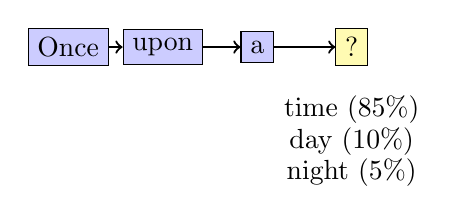
\begin{tikzpicture}[scale=0.8]
        % Input sequence
        \node[draw, fill=blue!20] (w1) at (0,0) {Once};
        \node[draw, fill=blue!20] (w2) at (1.5,0) {upon};
        \node[draw, fill=blue!20] (w3) at (3,0) {a};
        \node[draw, fill=yellow!30] (w4) at (4.5,0) {?};
        
        % Arrows showing prediction
        \draw[->, thick] (w1) -- (w2);
        \draw[->, thick] (w2) -- (w3);
        \draw[->, thick] (w3) -- (w4);
        
        % Prediction options
        \node at (4.5,-1) {time (85\%)};
        \node at (4.5,-1.5) {day (10\%)};
        \node at (4.5,-2) {night (5\%)};
    \end{tikzpicture}
    
    \vspace{0.5em}
    \textbf{Like autocomplete on steroids:}
    \begin{enumerate}
        \item Read text left to right
        \item Predict next word
        \item Use only what came before
        \item Keep going to generate text
    \end{enumerate}
    
    \column{0.5\textwidth}
    \textbf{GPT vs BERT:}
    
    \begin{center}
    \includegraphics[width=\textwidth]{../figures/bert_vs_gpt_architecture.pdf}
    \end{center}
    
    \begin{realworld}
    ChatGPT = GPT trained to have conversations. It's predicting the next word, one at a time, thousands of times per second!
    \end{realworld}
    \end{columns}
\end{frame}

% Visual comparison slide
\begin{frame}[t]{BERT vs GPT: Head-to-Head}
    \begin{center}
    \begin{tabular}{|l|c|c|}
    \hline
    \textbf{Feature} & \textbf{BERT} & \textbf{GPT} \\
    \hline
    \hline
    Direction & Bidirectional $\leftrightarrow$ & Left-to-right $\rightarrow$ \\
    \hline
    Training & Fill blanks & Predict next \\
    \hline
    Strength & Understanding & Generation \\
    \hline
    Best for & Classification & Text creation \\
    \hline
    Example & Sentiment analysis & ChatGPT \\
    \hline
    Speed & Faster for analysis & Slower (sequential) \\
    \hline
    Context & Sees everything & Only sees past \\
    \hline
    \end{tabular}
    \end{center}
    
    \vspace{0.5em}
    \begin{columns}
    \column{0.5\textwidth}
    \begin{intuition}
    BERT = Reading comprehension expert\\
    GPT = Creative writing expert
    \end{intuition}
    
    \column{0.5\textwidth}
    \begin{checkpoint}
    Remember: BERT for understanding, GPT for generating!
    \end{checkpoint}
    \end{columns}
\end{frame}

% Fine-tuning visualization
\begin{frame}[t]{Fine-tuning: Teaching New Tricks}
    \begin{columns}
    \column{0.6\textwidth}
    \begin{center}
    \includegraphics[width=\textwidth]{../figures/fine_tuning_process.pdf}
    \end{center}
    
    \textbf{The fine-tuning advantage:}
    \begin{itemize}
        \item Start with language knowledge
        \item Add task-specific skills
        \item 10x faster convergence
        \item Need less data
    \end{itemize}
    
    \column{0.4\textwidth}
    \textbf{Like learning a specialty:}
    
    \begin{enumerate}
        \item Pre-training = Medical school
        \item Fine-tuning = Specialization
        \begin{itemize}
            \item Cardiology
            \item Neurology
            \item Pediatrics
        \end{itemize}
    \end{enumerate}
    
    \begin{misconception}
    ``Fine-tuning erases pre-training'' - No! It adds a thin layer of task-specific knowledge on top.
    \end{misconception}
    \end{columns}
\end{frame}

% Model zoo
\begin{frame}[t]{The Model Zoo: Choose Your Fighter!}
    \begin{center}
    \includegraphics[width=0.9\textwidth]{../figures/model_size_comparison.pdf}
    \end{center}
    
    \begin{checkpoint}
    Bigger isn't always better! Choose based on:
    \begin{itemize}
        \item Your task complexity
        \item Available computing power
        \item Response time requirements
    \end{itemize}
    \end{checkpoint}
\end{frame}

% Decision tree
\begin{frame}[t]{Which Model Should You Use?}
    \begin{center}
    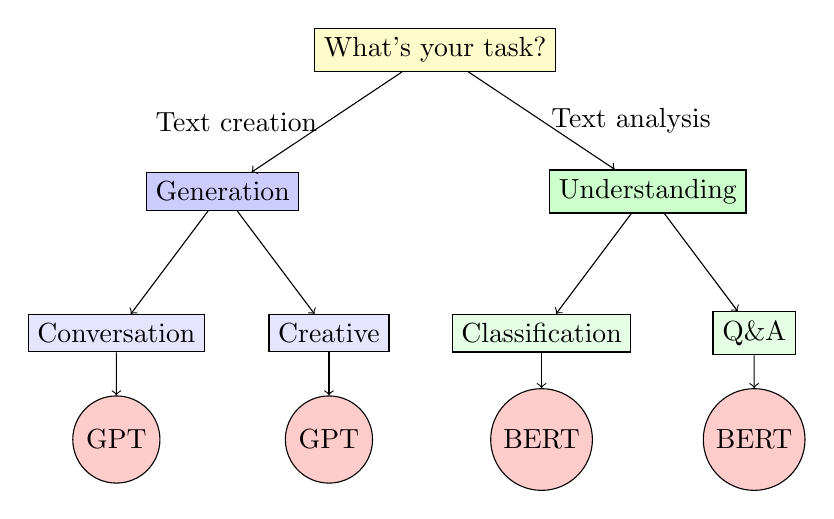
\begin{tikzpicture}[scale=0.9]
        % Root
        \node[draw, rectangle, fill=yellow!20] (root) at (0,0) {What's your task?};
        
        % Level 1
        \node[draw, rectangle, fill=blue!20] (gen) at (-3,-2) {Generation};
        \node[draw, rectangle, fill=green!20] (und) at (3,-2) {Understanding};
        
        % Level 2 - Generation
        \node[draw, rectangle, fill=blue!10] (chat) at (-4.5,-4) {Conversation};
        \node[draw, rectangle, fill=blue!10] (story) at (-1.5,-4) {Creative};
        
        % Level 2 - Understanding
        \node[draw, rectangle, fill=green!10] (class) at (1.5,-4) {Classification};
        \node[draw, rectangle, fill=green!10] (qa) at (4.5,-4) {Q\&A};
        
        % Recommendations
        \node[draw, circle, fill=red!20] (gpt) at (-4.5,-5.5) {GPT};
        \node[draw, circle, fill=red!20] (gpt2) at (-1.5,-5.5) {GPT};
        \node[draw, circle, fill=red!20] (bert) at (1.5,-5.5) {BERT};
        \node[draw, circle, fill=red!20] (bert2) at (4.5,-5.5) {BERT};
        
        % Connections
        \draw[->] (root) -- (gen) node[midway,left] {Text creation};
        \draw[->] (root) -- (und) node[midway,right] {Text analysis};
        \draw[->] (gen) -- (chat);
        \draw[->] (gen) -- (story);
        \draw[->] (und) -- (class);
        \draw[->] (und) -- (qa);
        \draw[->] (chat) -- (gpt);
        \draw[->] (story) -- (gpt2);
        \draw[->] (class) -- (bert);
        \draw[->] (qa) -- (bert2);
    \end{tikzpicture}
    \end{center}
    
    \begin{realworld}
    Real applications: Gmail autocomplete (GPT-style), Google search understanding (BERT-style)
    \end{realworld}
\end{frame}

% Timeline
\begin{frame}[t]{The Evolution: From ELMo to GPT-4}
    \begin{center}
    \includegraphics[width=0.9\textwidth]{../figures/pretraining_timeline.pdf}
    \end{center}
    
    \begin{intuition}
    Notice the exponential growth! Each generation is 10x bigger, following Moore's Law for AI.
    \end{intuition}
\end{frame}

% Hands-on code example
\begin{frame}[fragile]{Let's Code: Using Pre-trained BERT}
    \begin{lstlisting}[language=Python]
# Super simple BERT usage
from transformers import pipeline

# Load pre-trained BERT for sentiment
classifier = pipeline("sentiment-analysis")

# That's it! Now use it:
result = classifier("I love this NLP course!")
print(result)
# Output: [{'label': 'POSITIVE', 'score': 0.99}]

# Fill-in-the-blank with BERT
fill_mask = pipeline("fill-mask")
result = fill_mask("The course is [MASK] interesting.")
print(result[0])
# Output: {'token_str': 'very', 'score': 0.85}
    \end{lstlisting}
    
    \begin{checkpoint}
    3 lines of code vs 3 months of training from scratch!
    \end{checkpoint}
\end{frame}

% Environmental awareness
\begin{frame}[t]{The Carbon Footprint Reality}
    \begin{columns}
    \column{0.5\textwidth}
    \textbf{Training costs:}
    \begin{itemize}
        \item GPT-3: 1,287 MWh of electricity
        \item = 552 tons of CO2
        \item = 120 cars for a year
    \end{itemize}
    
    \vspace{0.5em}
    \textbf{Why this matters:}
    \begin{itemize}
        \item Use pre-trained when possible
        \item Don't train from scratch
        \item Share your models
        \item Consider efficiency
    \end{itemize}
    
    \column{0.5\textwidth}
    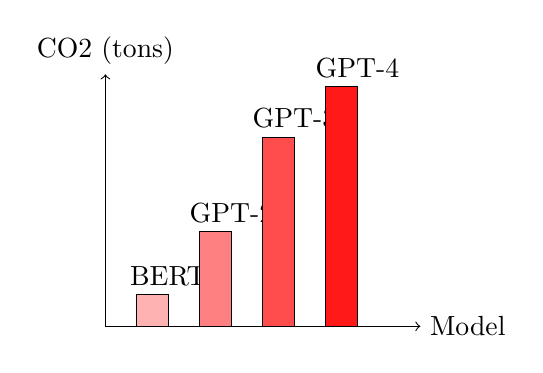
\begin{tikzpicture}[scale=0.8]
        % Bar chart of CO2 emissions
        \draw[->] (0,0) -- (5,0) node[right] {Model};
        \draw[->] (0,0) -- (0,4) node[above] {CO2 (tons)};
        
        \draw[fill=red!30] (0.5,0) rectangle (1,0.5) node[above] {BERT};
        \draw[fill=red!50] (1.5,0) rectangle (2,1.5) node[above] {GPT-2};
        \draw[fill=red!70] (2.5,0) rectangle (3,3) node[above] {GPT-3};
        \draw[fill=red!90] (3.5,0) rectangle (4,3.8) node[above] {GPT-4};
    \end{tikzpicture}
    
    \begin{realworld}
    One GPT-3 training run = Flying from NY to SF 400 times!
    \end{realworld}
    \end{columns}
\end{frame}

% Exercise slide
\begin{frame}[t]{Your Turn: Hands-On Exercise}
    \textbf{Exercise: Fine-tune BERT for Movie Reviews}
    
    \begin{enumerate}
        \item Load pre-trained BERT-base
        \item Prepare IMDB movie review dataset
        \item Fine-tune for 3 epochs
        \item Compare with training from scratch
    \end{enumerate}
    
    \vspace{0.5em}
    \textbf{Expected results:}
    \begin{itemize}
        \item Fine-tuned BERT: 92\% accuracy in 10 minutes
        \item From scratch: 75\% accuracy in 2 hours
    \end{itemize}
    
    \vspace{0.5em}
    \begin{columns}
    \column{0.5\textwidth}
    \begin{checkpoint}
    Use Google Colab for free GPU access!
    \end{checkpoint}
    
    \column{0.5\textwidth}
    \begin{intuition}
    Fine-tuning is like teaching a professor a new course vs teaching a toddler everything from scratch.
    \end{intuition}
    \end{columns}
\end{frame}

% Key takeaways
\begin{frame}[t]{Key Takeaways: What to Remember}
    \begin{columns}
    \column{0.5\textwidth}
    \textbf{The Big Ideas:}
    \begin{enumerate}
        \item \textbf{Pre-training} = Learning language once
        \item \textbf{Fine-tuning} = Adapting to your task
        \item \textbf{BERT} = Bidirectional understanding
        \item \textbf{GPT} = Sequential generation
        \item \textbf{Transfer learning} = Reuse knowledge
    \end{enumerate}
    
    \column{0.5\textwidth}
    \textbf{Practical Tips:}
    \begin{itemize}
        \item Never train from scratch
        \item Start with smallest model that works
        \item Use Hugging Face for easy access
        \item Fine-tune on your specific domain
        \item Monitor environmental impact
    \end{itemize}
    \end{columns}
    
    \vspace{0.5em}
    \begin{realworld}
    Every major AI application today uses pre-trained models: ChatGPT, Google Search, Grammarly, GitHub Copilot, and more!
    \end{realworld}
\end{frame}

% Future directions
\begin{frame}[t]{The Future: What's Next?}
    \textbf{Current Frontiers (2024):}
    \begin{itemize}
        \item \textbf{Multimodal:} Text + Images + Audio (GPT-4V)
        \item \textbf{Efficient:} Smaller, faster models (Llama, Phi)
        \item \textbf{Specialized:} Domain-specific models (BloombergGPT)
        \item \textbf{Aligned:} Following human values (Claude)
    \end{itemize}
    
    \vspace{0.5em}
    \textbf{Next Week Preview:}
    \begin{itemize}
        \item Advanced transformer architectures
        \item Efficient transformers
        \item Scaling laws
        \item Emergent abilities
    \end{itemize}
    
    \begin{checkpoint}
    The field moves fast! What you learn today will evolve, but the core concepts remain.
    \end{checkpoint}
\end{frame}

% Summary slide
\begin{frame}[t]{Summary: From Zero to Hero}
    \begin{center}
    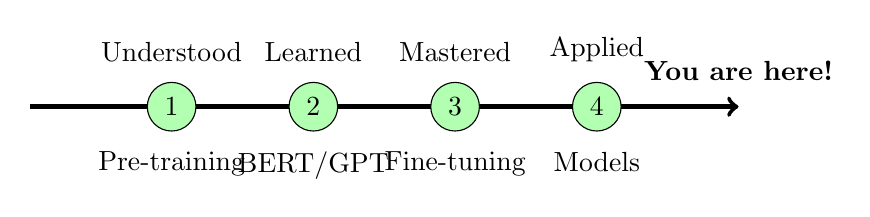
\begin{tikzpicture}[scale=0.9]
        % Journey path
        \draw[ultra thick, ->] (0,0) -- (10,0);
        
        % Milestones
        \node[draw, circle, fill=green!30] (m1) at (2,0) {1};
        \node[above] at (2,0.5) {Understood};
        \node[below] at (2,-0.5) {Pre-training};
        
        \node[draw, circle, fill=green!30] (m2) at (4,0) {2};
        \node[above] at (4,0.5) {Learned};
        \node[below] at (4,-0.5) {BERT/GPT};
        
        \node[draw, circle, fill=green!30] (m3) at (6,0) {3};
        \node[above] at (6,0.5) {Mastered};
        \node[below] at (6,-0.5) {Fine-tuning};
        
        \node[draw, circle, fill=green!30] (m4) at (8,0) {4};
        \node[above] at (8,0.5) {Applied};
        \node[below] at (8,-0.5) {Models};
        
        \node at (10,0.5) {\textbf{You are here!}};
    \end{tikzpicture}
    \end{center}
    
    \vspace{1em}
    \begin{intuition}
    You now understand the technology behind ChatGPT, Google Search, and modern AI. That's huge!
    \end{intuition}
\end{frame}

\end{document}